\RequirePackage{iftex}
\ifPDFTeX
  \documentclass{article}
  \usepackage[utf8]{inputenc}
  \usepackage[T1]{fontenc}
  \usepackage{CJKutf8}
\else
  \documentclass[UTF8]{ctexart}
\fi

\usepackage[a4paper,margin=2.5cm]{geometry}
\usepackage{amsmath,amssymb}
\usepackage{amsthm}
\usepackage{booktabs}
\usepackage{amsfonts}
\usepackage{nicefrac}
\usepackage{microtype}
\usepackage[table]{xcolor}
\usepackage{multirow,array}
\usepackage[final]{graphicx}
\usepackage{enumitem}
\usepackage{float}
\usepackage{subcaption}
\usepackage{tabularx}
\usepackage{hyperref}
\usepackage{url}
\captionsetup[subfigure]{font=normalsize,labelfont=bf,textfont=bf,justification=centering,singlelinecheck=false,skip=2pt}

\newtheorem{theorem}{定理}[section]
\newtheorem{corollary}[theorem]{推论}

\newcommand{\tbd}{待补充}
\providecommand{\answerYes}[1]{\textbf{Yes}}
\providecommand{\answerNo}[1]{\textbf{No}}
\providecommand{\answerNA}[1]{\textbf{N/A}}
\providecommand{\answerTODO}[1]{\textbf{TODO}}
\providecommand{\justificationTODO}[1]{\textbf{TODO}}
\definecolor{improvblue}{RGB}{236,242,255}
\newcommand{\impcell}[1]{\cellcolor{improvblue}#1}
\newcommand{\impblank}{\cellcolor{improvblue}}
\newcommand{\impheaderbox}{\begingroup\setlength{\fboxsep}{0pt}\colorbox{improvblue}{\parbox[c][4.9ex][c]{1.20cm}{\centering\textbf{Improv.}}}\endgroup}
\newcommand{\impfullhead}{\multicolumn{1}{>{\columncolor{improvblue}[0pt][0pt]\centering\arraybackslash}m{1.20cm}}{\textbf{Improv.}}}
\newcommand{\impfullcell}[1]{\multicolumn{1}{>{\columncolor{improvblue}[0pt][0pt]\centering\arraybackslash}m{1.20cm}}{#1}}
\newcommand{\impfullblank}{\multicolumn{1}{>{\columncolor{improvblue}[0pt][0pt]\centering\arraybackslash}m{1.20cm}}{}}
\newcommand{\impheadmulti}{\multirow{2}{*}[-0.35ex]{\textbf{Improv.}}}
\newcolumntype{I}{>{\columncolor{improvblue}[\tabcolsep][\tabcolsep]\centering\arraybackslash}m{1.20cm}}

\title{序列去哪了？通过大-小模型协同重塑空间以提升 LLM 的序列理解能力}
\author{}
\date{}

\begin{document}
\ifPDFTeX
\begin{CJK*}{UTF8}{gbsn}
\fi

\maketitle

\begin{abstract}
大语言模型（LLMs）凭借强大的语义建模能力，正逐渐成为推荐系统的重要基础模型。因此，越来越多的研究开始尝试联合建模 LLM 与序列推荐信号。然而，现有方法大多停留在“把特征接入 LLM”这一层面，而没有真正建立协同表示与语言语义之间的深层耦合。我们认为，协同过滤空间与 LLM 语义空间之间存在一个\emph{语义-序列异构鸿沟}（Semantic-Sequential Heterogeneity Gap, SSHG）。这种上游不兼容性会在跨空间注入过程中削弱可迁移的序列线索，并最终表现为不稳定的序列利用。为此，我们提出 \textbf{EchoRec}，一个分阶段的大-小模型协同框架：首先利用冻结的 LLM 通过\emph{语义对齐对比预训练}（Semantic-Aligned Contrastive Pre-training, SACP）将序列教师重塑为更干净的序列空间，再通过\emph{序列注入}（Sequence Injection, SI）把提纯后的序列结构迁移到 LLM 中。在当前共享 benchmark 设置下，EchoRec 在可直接比较的 LLM4Rec 方法中取得了 SOTA 表现。
\end{abstract}

\section{引言}
\label{sec:introduction}

随着文本理解、上下文建模与开放域推理能力的快速提升，大语言模型（LLMs）正日益被视为推荐系统的潜在基础模型~\cite{lin2025survey,zhao2024era}。其强大的语义能力与统一的建模接口推动了大量工作尝试将 LLM 与序列推荐信号结合起来。然而，在序列推荐中，\emph{接收到}用户历史并不等价于\emph{可靠地利用}了这段历史。当协同信号只是作为附加特征被注入，而没有与语言语义形成深层耦合时，模型更可能依赖浅层上下文线索，而不是稳定的行为依赖；近期关于 LLM 推荐模型顺序敏感性弱与上下文偏置的诊断工作也支持这一判断~\cite{kim2025lost,wang2026contextbias}。因此，一个核心问题是：如何在保留 LLM 语义优势的同时，为 LLM 推荐注入可靠的序列归纳偏置。

早期工作主要通过提示、轻量调优或显式推理框架把 LLM 直接适配到推荐任务中~\cite{bao2023tallrec,yu2026thinkrec}。随着纯文本适配方案的局限逐渐显现，后续研究开始把协同知识重新带回推荐流程：要么将 LLM 与预训练序列推荐器对齐~\cite{liao2024llara,kim2024allmrec}，要么把协同信号直接注入 LLM 上下文~\cite{zhang2025collm,zheng2024lcrec,hong2025eagerllm,kim2025lost}。另一条路线则把 LLM 放在在线决策环之外，将其作为语义编码器或关系提供器来增强小型序列模型~\cite{ren2024rlmrec,yang2024lrd,liu2024llmesr,cui2025sracl}。这些方法在 LLM 所处位置与协同特征的使用方式上各不相同，但它们共享一个隐含前提：协同信号能够以可控代价与 LLM 语义协同起来，并且其中携带的序列结构能够在迁移过程中不被严重扭曲。

我们认为，这一前提往往过于乐观，因为原始协同空间与 LLM 语义空间遵循着截然不同的邻域规则。前者主要由 ID 共现、流行度偏置与稀疏交互噪声塑形，后者则由文本语义与世界知识组织。我们将这种结构性鸿沟称为\emph{语义-序列异构鸿沟}（SSHG）。具体而言，SSHG 主要表现为两类与注入直接相关的错配：其一是\emph{局部语义度量错配}，即冻结 LLM 空间中的语义近邻无法在原始序列推荐空间中得到保留；其二是\emph{语义邻域拓扑碎片化}，即语义相近的用户或序列未能在协同空间中形成连贯的局部区域。近期关于 token-level 协同对齐、基于 LLM 的视图增强与跨模态对比学习的工作，也都表明这两类空间在局部规则上并不天然兼容~\cite{lin2026tca4rec,lu2025cllmrec,xu2024cmclrec}。因此，当一个轻量投影器被迫同时承担去噪、局部结构修复与跨空间对齐时，可迁移的序列线索很可能在被 LLM 吸收之前就已经被削弱。近期诊断工作也报告了相同的下游症状：LLM 推荐模型可能依赖捷径上下文或浅层推理，而不是稳定的序列依赖~\cite{kim2025lost,wang2026contextbias,yu2026thinkrec}。

从跨空间对齐的角度看，注入效率高度依赖于序列空间的局部结构是否与目标语义空间兼容。受到近期大-小模型协同推荐研究的启发~\cite{zhang2026crossscale,lv2025lsc4rec}，我们进一步认为，“LLM 增强序列推荐器”和“序列推荐器增强 LLM”不应被视为两条彼此分离的路线。如果能在注入之前先重塑教师空间，使其局部邻域结构更贴近 LLM 语义空间，那么后续映射所需的结构扭曲就会显著下降。换言之，前一条路线可以为协同空间提供语义先验并完成净化，后一条路线则可以把更高质量的序列模式反馈给在线 LLM。

基于这一观察，我们提出 EchoRec，一个分阶段的大-小模型协同框架。其核心思想是\emph{先重塑，再注入}。冻结 LLM 首先构建离线语义资产，并据此通过语义对齐对比预训练（SACP）将协同教师空间重塑为更干净、更可迁移的序列空间；随后，序列注入（SI）在显式教师对齐约束下，把提炼后的序列模式迁移到 LLM 中。通过这种方式，EchoRec 将“LLM 增强序列推荐器”与“序列推荐器反向增强 LLM”统一在同一个闭环之中。

本文的主要贡献如下：
\begin{itemize}[leftmargin=1.5em]
\item 我们形式化定义了 LLM 增强序列推荐中的\emph{语义-序列异构鸿沟}（SSHG），并解释了这种上游错配如何导致注入失真与不稳定的序列利用。
\item 我们提出 EchoRec 这一分阶段框架，其中 SACP 先重塑教师空间，随后 SI 在显式教师对齐下将提纯后的序列模式迁移到 LLM。
\item 我们给出了跨空间注入下序列保持的分布视角，并证明在显式宿主兼容性假设下，教师侧错配与注入时表示漂移共同上界序列保持误差。
\item 我们在当前共享 benchmark 上验证了 EchoRec 对强基线的稳定优势，并进一步表明其在序列扰动下具有更好的稳定性。
\end{itemize}

\section{预备知识}
\label{sec:preliminary}

记 $\mathcal{U}$ 为用户集合，$\mathcal{I}$ 为物品集合。对于任意用户 $u\in\mathcal{U}$，其按时间顺序排列的观测交互历史记为 $S_u=[i_1^u,i_2^u,\dots,i_{n_u-1}^u]$，其中 $i_t^u\in\mathcal{I}$。序列推荐的目标是根据历史序列 $S_u$ 预测下一次交互物品 $y_u=i_{n_u}^u$，即
\begin{equation}
\arg\max_{i \in \mathcal{I}} P(y_u=i \mid S_u).
\end{equation}
其中，$S_u$ 表示观测到的历史，$y_u$ 表示待预测的下一物品。传统序列模型如 GRU4Rec、SASRec 与 BERT4Rec~\cite{hidasi2016gru4rec,kang2018sasrec,sun2019bert4rec}因此具备显式的序列归纳偏置，但其表示空间依然主要由 ID 共现关系主导。

\subsection{LLM4Rec 设定}

本文中的 \emph{LLM4Rec} 指的是保留 LLM 在在线决策环中，并由其直接产生推荐输出的方法。在这一设定下，用户历史通常以文本 prompt 或 soft prompt 的形式输入 LLM。对于特征注入类方法，小型推荐器的协同表示会先映射到 LLM 隐空间，再作为上下文条件参与推理。已有诊断证据~\cite{kim2025lost} 表明，现有 LLM4Rec 模型对序列扰动的敏感性有限，这意味着“输入了历史”并不等价于“稳定利用了历史中的序列信息”。

\subsection{语义-序列异构鸿沟（SSHG）}

记传统序列推荐器学习得到的协同表示空间为 $\mathcal{S}_{CF}$，记 LLM 内在的语义空间为 $\mathcal{S}_{LLM}$。前者主要由 ID 共现统计塑形，后者则由语义逻辑与语言先验组织。本文将这两类空间之间、并且会影响跨空间注入的系统性错配定义为\emph{语义-序列异构鸿沟}（SSHG）。具体来说，SSHG 包含两个耦合方面：\emph{局部语义度量错配}，即由 $\mathcal{S}_{CF}$ 诱导的近邻结构与由 $\mathcal{S}_{LLM}$ 诱导的近邻结构不一致；以及\emph{语义邻域拓扑碎片化}，即语义相近的用户或序列未能在 $\mathcal{S}_{CF}$ 中形成连贯的局部区域。

给定训练集 $\mathcal{D}=\{(S_u,y_u)\}_{u=1}^{|\mathcal{U}|}$，通用的序列推荐目标可写为
\begin{equation}
\min_{\Theta}\mathcal{L}_{rec}
=
-\frac{1}{|\mathcal{D}|}\sum_{(S_u,y_u)\in\mathcal{D}}
\log P_{\Theta}(y_u\mid S_u).
\end{equation}
其中，$\mathcal{D}$ 表示训练集，$\Theta$ 表示待学习参数，$\mathcal{L}_{rec}$ 表示通用的下一物品推荐损失。后文中，EchoRec 会分别在教师侧和 LLM 侧基于这一目标施加不同的结构约束。

\section{方法}
\label{sec:method}

\subsection{整体概览}

给定用户集合 $\mathcal{U}$、物品集合 $\mathcal{I}$ 以及用户 $u$ 的时间有序交互序列 $S_u=[i_1^u,i_2^u,\dots,i_{T_u}^u]$，我们的目标是预测下一物品 $y_u$。EchoRec 遵循一个两阶段的大-小模型协同流程：冻结 LLM 先提供语义资产以重塑序列教师，增强后的教师再把提纯的序列结构迁移回 LLM。整个方法包含三个部分：语义资产准备、教师侧语义对齐对比预训练（SACP）以及结构感知的序列注入（SI）。记冻结语义编码器为 $E_{llm}$，原始序列骨干为 $G_{sr}$，增强教师为 $G_{sr}^{+}$；同时记增强物品表、跨模态投影器、教师侧对齐映射器以及 LLM 侧用户/物品头分别为 $E_{item}^{+}$、$\Pi_{\phi}$、$M_{\psi}$、$f_u$ 和 $f_i$。

全文中我们使用三类表示：离线语义资产 $\mathbf{e}^{sem}\in\mathbb{R}^{d_{sem}}$、教师空间中的协同表示 $\mathbf{z}^{+}\in\mathbb{R}^{d_s}$，以及 LLM 侧检索子空间中的表示 $\hat{\mathbf{u}}, \hat{\mathbf{v}}\in\mathbb{R}^{d_r}$。在实现上，$\Pi_{\phi}$ 将教师物品嵌入投影到 LLM 隐空间，$f_u$ 与 $f_i$ 将 LLM 锚点状态映射到统一检索空间，而 $M_{\psi}$ 将教师用户表示映射到同一检索空间用于对齐。

\begin{figure*}[!t]
\centering
\IfFileExists{figure/echorec_architecture.pdf}{%
  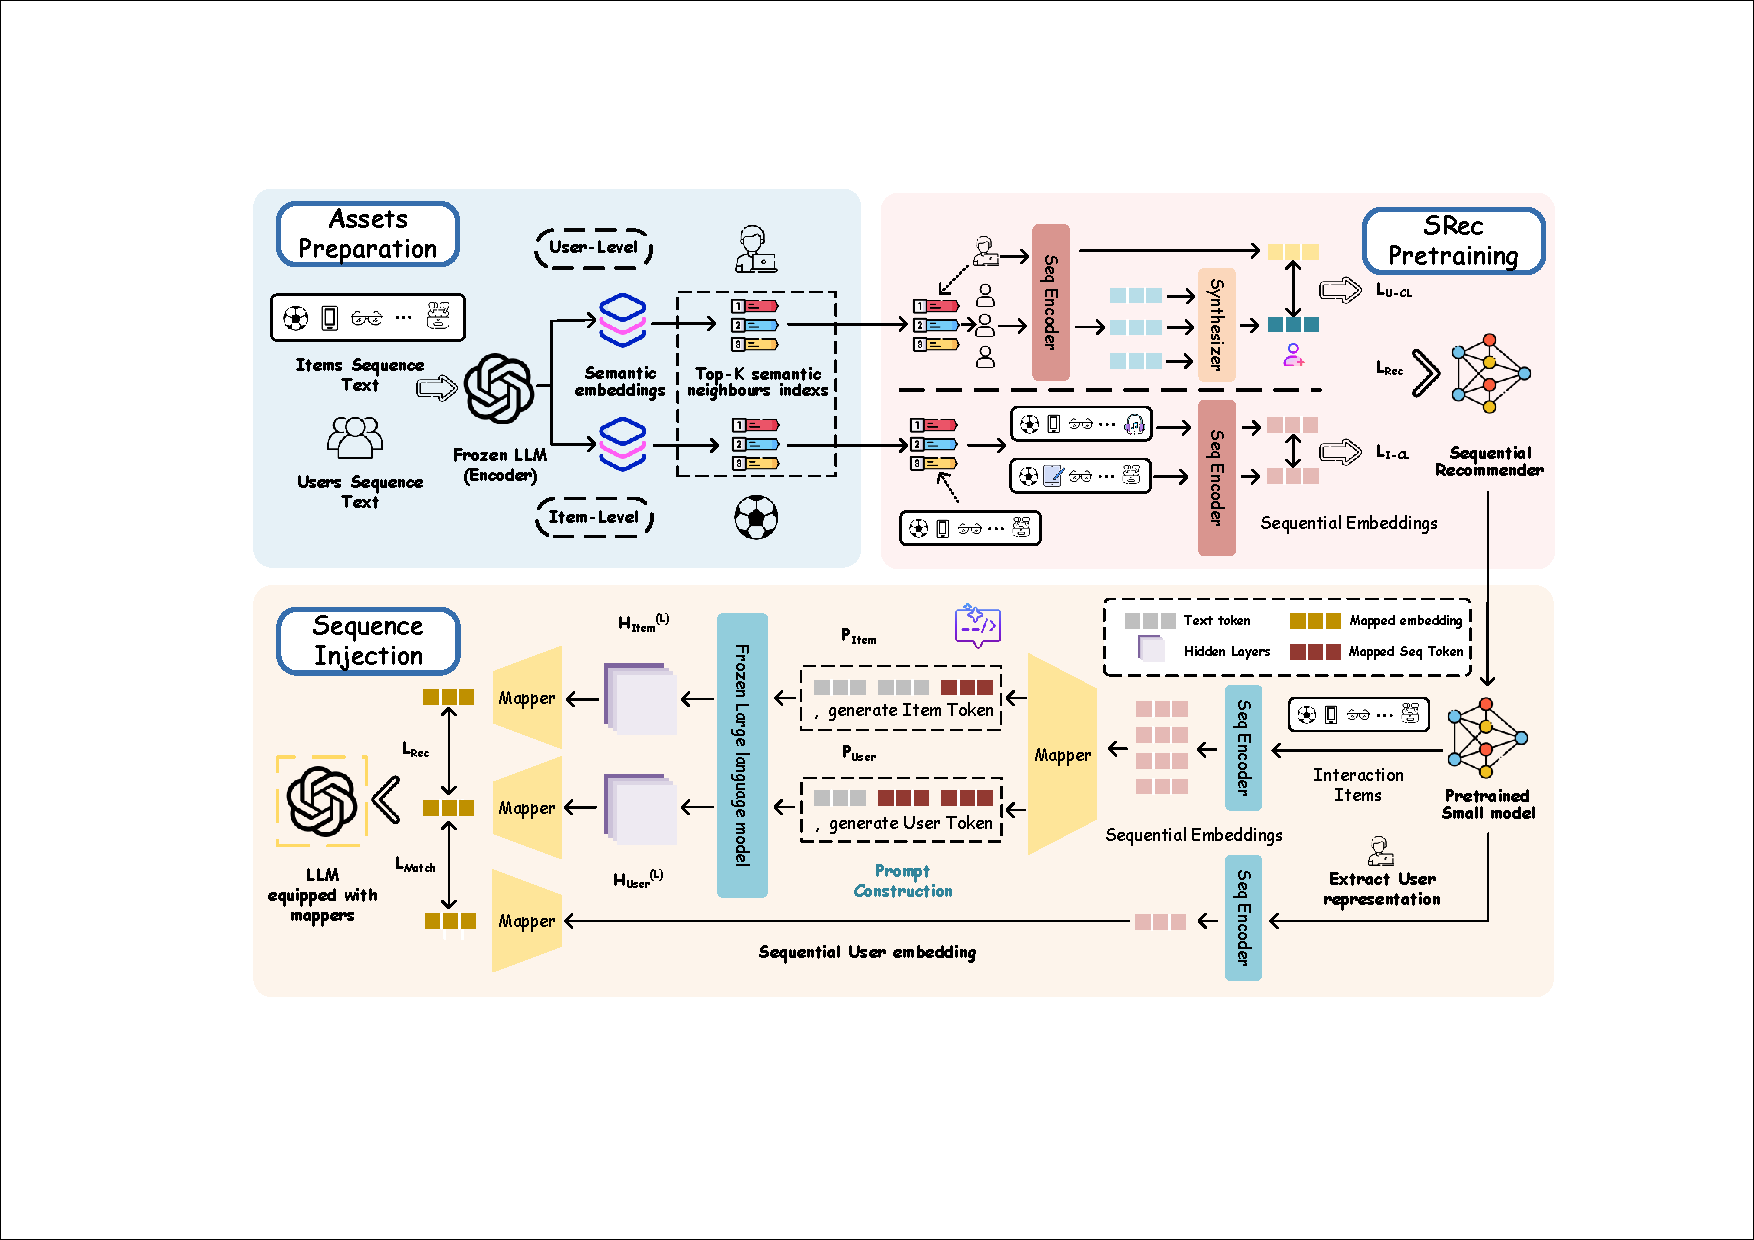
\includegraphics[width=\textwidth,trim=122 110 96 85,clip]{figure/echorec_architecture.pdf}%
}{%
  \IfFileExists{echorec_architecture.pdf}{%
    
\includegraphics[width=\textwidth,trim=122 110 96 85,clip]{echorec_architecture.pdf}%
  }{%
    \IfFileExists{\detokenize{docs/EchoRec 架构图0415_cropped.pdf}}{%
      
\includegraphics[width=\textwidth]{\detokenize{docs/EchoRec 架构图0415_cropped.pdf}}%
    }{%
      \IfFileExists{\detokenize{docs/EchoRec 架构图0415.pdf}}{%
        
\includegraphics[width=\textwidth]{\detokenize{docs/EchoRec 架构图0415.pdf}}%
      }{%
        \fbox{\rule{0pt}{2.7in}\rule{0.95\textwidth}{0pt}}%
      }%
    }%
  }%
}%
\caption{EchoRec 的总体架构。冻结 LLM 首先构建离线语义资产与语义邻域索引，并据此在阶段一通过语义对齐对比预训练（SACP）重塑教师协同空间；随后，增强教师输出提纯后的序列嵌入，在阶段二通过序列注入（SI）把投影后的协同物品嵌入注入冻结 LLM，并与教师侧用户表示进行对齐。}
\label{fig:echorec_architecture}
\end{figure*}

\subsection{语义资产准备}

在阶段一中，EchoRec 仅使用冻结 LLM 来构建离线语义资产。对于每个物品 $i$，我们根据标题与可用描述构建文本描述 $x_i$；对于每条用户序列，则构建文本化历史 $x_u^{seq}$。设冻结 LLM 最后一层隐藏输出为 $\mathbf{H}^{(L)}(x)\in\mathbb{R}^{L_x\times d_{sem}}$，其 attention mask 为 $\mathbf{m}\in\{0,1\}^{L_x}$，则我们采用 masked mean pooling 得到语义向量：
\begin{equation}
\mathrm{Enc}_{sem}(x)=
\mathrm{Norm}\!\left(
\frac{\sum_{t=1}^{L_x} m_t \mathbf{H}^{(L)}_t(x)}
{\sum_{t=1}^{L_x} m_t}
\right).
\end{equation}
其中，$L_x$ 为输入 $x$ 的 token 长度，$m_t$ 为位置 $t$ 的 mask 值，$\mathrm{Norm}(\cdot)$ 表示向量归一化。我们将节点 $v$ 的语义向量记为 $\mathbf{e}_v^{sem}$。对任意两个语义节点 $v$ 与 $v'$，其相似度定义为
\begin{equation}
s^{sem}(v,v')
=
\frac{(\mathbf{e}_v^{sem})^\top \mathbf{e}_{v'}^{sem}}
{\|\mathbf{e}_v^{sem}\|_2\|\mathbf{e}_{v'}^{sem}\|_2},
\end{equation}
对应的 Top-$K$ 语义邻域定义为
\begin{equation}
\mathcal{N}_{sem}^{K}(v)
=
\operatorname*{TopK}_{v'\in\mathcal{V}\setminus\{v\}}
\ s^{sem}(v,v').
\end{equation}
其中，$K$ 表示邻域大小，$\mathcal{V}$ 表示构建语义图时采用的节点全集。我们对用户与物品都执行这一构造，并在后续训练中保持这些语义资产冻结，作为稳定的语义参考系。

\subsection{阶段一：语义对齐对比预训练（SACP）}

阶段一的目标是将原始协同空间重塑为更适合跨模态迁移的教师空间。我们保留标准序列监督，同时引入两类语义约束：item-level 分支面向局部语义度量错配，user-level 分支面向语义邻域拓扑碎片化。

\subsubsection{序列表征与推荐目标}

设 $\mathbf{z}_u^{raw}\in\mathbb{R}^{d_s}$ 为序列编码器 $G_{sr}$ 对序列 $S_u$ 的最后位置输出。为了适配对比学习，我们引入一个轻量投影头，并得到
\begin{equation}
\mathbf{r}_u=g_{\omega}(\mathbf{z}_u^{raw}).
\end{equation}
其中，$\mathbf{r}_u$ 为用于对比学习的投影后序列表征，$g_{\omega}$ 为参数为 $\omega$ 的轻量投影头。阶段一仍优化标准的下一物品预测目标：
\begin{equation}
\mathcal{L}_{rec}^{sr}
=-\frac{1}{|\mathcal{B}|}\sum_{u\in\mathcal{B}}
\log
\frac{\exp\big((\mathbf{z}_u^{raw})^\top \mathbf{q}_{y_u}\big)}
{\sum_{j\in\mathcal I}\exp\big((\mathbf{z}_u^{raw})^\top \mathbf{q}_{j}\big)}.
\end{equation}
其中，$\mathcal{B}$ 为 minibatch，$y_u$ 为用户 $u$ 的真实下一物品，$\mathbf{q}_j$ 为物品 $j$ 的嵌入。该项保证增强后的教师仍保留序列判别能力，而不会被纯语义约束拉向一个脱离推荐目标的空间。

\subsubsection{Item-level 语义扰动一致性}

为了在不破坏核心序列语义的前提下引入可控扰动，我们不采用完全随机的 token 替换，而是从冻结语义邻域中采样语义相近物品，构建两条增强视图 $\tilde{S}_u^{(1)}$ 与 $\tilde{S}_u^{(2)}$。将两条视图重新编码并经过投影头后，我们优化标准的 InfoNCE 目标：
\begin{equation}
\mathcal{L}_{i\text{-}cl}
=-\frac{1}{|\mathcal{B}|}\sum_{u\in\mathcal{B}}
\log
\frac{\exp(\mathrm{sim}(\mathbf{r}_u^{(1)},\mathbf{r}_u^{(2)})/\tau_s)}
{\sum_{v\in\mathcal{B}}
\exp(\mathrm{sim}(\mathbf{r}_u^{(1)},\mathbf{r}_v^{(2)})/\tau_s)}.
\end{equation}
其中，$\mathbf{r}_u^{(1)}$ 与 $\mathbf{r}_u^{(2)}$ 分别表示同一序列两条增强视图的投影表示，$\mathbf{r}_v^{(2)}$ 表示 minibatch 中另一条序列 $v$ 的第二视图投影表示，$\mathrm{sim}(\cdot,\cdot)$ 表示余弦相似度，$\tau_s$ 为对比温度。该分支鼓励模型对“语义相近但 ID 不完全相同”的局部扰动作出一致响应，从而使序列推荐空间中的局部相似性不再过度依赖精确 ID 重合，并更接近冻结语义空间定义的局部度量。

\subsubsection{User-level 语义邻域聚合}

仅靠 item-level 增强还不足以刻画用户层面的语义组织，因此我们进一步引入 user-level 语义邻域聚合分支。对于每个用户 $u$，记其语义邻域为 $\mathcal{N}_{u,\mathrm{sem}}^K:=\mathcal{N}_{sem}^{K}(u)$，我们对其中邻居进行编码，并根据冻结语义资产计算语义引导的混合权重
\begin{equation}
w_{u,v}
=
\frac{\exp(\kappa(\mathbf{e}_u^{sem},\mathbf{e}_v^{sem}))}
{\sum_{v'\in\mathcal{N}_{u,\mathrm{sem}}^K}\exp(\kappa(\mathbf{e}_u^{sem},\mathbf{e}_{v'}^{sem}))},
\end{equation}
其中，$\kappa(\cdot,\cdot)$ 是作用于冻结语义资产上的轻量可学习打分函数。相应的混合邻域表示为
\begin{equation}
\bar{\mathbf{r}}_u=\sum_{v\in\mathcal{N}_{u,\mathrm{sem}}^K}w_{u,v}\mathbf{r}_{u,v}.
\end{equation}
其中，$\bar{\mathbf{r}}_u$ 为用户 $u$ 的语义邻域混合表示，$\mathbf{r}_{u,v}$ 为用户 $u$ 的语义邻居 $v$ 的投影表示。
随后，我们以该邻域表示为正样本目标，构造 user-level 对比对齐目标：
\begin{equation}
\mathcal{L}_{u\text{-}cl}
=-\frac{1}{|\mathcal{B}|}\sum_{u\in\mathcal{B}}
\log
\frac{\exp(\mathrm{sim}(\mathbf{r}_u,\bar{\mathbf{r}}_u)/\tau_s)}
{\sum_{v\in\mathcal{B}}
\exp(\mathrm{sim}(\mathbf{r}_u,\bar{\mathbf{r}}_v)/\tau_s)}.
\end{equation}
其中，$\bar{\mathbf{r}}_u$ 为上文定义的用户 $u$ 的语义邻域混合表示，$\bar{\mathbf{r}}_v$ 表示 minibatch 中另一位用户 $v$ 的对应混合表示，$\mathrm{sim}(\cdot,\cdot)$ 表示余弦相似度，$\tau_s$ 与 item-level 分支共用同一对比温度。该分支鼓励模型在语义相近用户区域内学习更平滑的决策边界，并减少重塑后序列推荐空间中的语义邻域碎片化。

\subsubsection{阶段一总体目标}

综合序列推荐监督与两类语义约束，阶段一总体目标为
\begin{equation}
\mathcal{L}_{\text{SACP}}
=
\mathcal{L}_{rec}^{sr}
+\lambda_u \mathcal{L}_{u\text{-}cl}
+\lambda_i \mathcal{L}_{i\text{-}cl}.
\end{equation}
其中，$\lambda_u$ 与 $\lambda_i$ 分别控制 user-level 与 item-level 语义约束的相对权重。优化完成后得到增强教师 $G_{sr}^{+}$。传递到阶段二的并不是对比头输出，而是重塑后的教师骨干本身。

\subsection{阶段二：结构感知的序列注入}

阶段二负责将增强教师中的序列知识迁移到 LLM。我们不强制点对点的隐藏状态匹配，而是要求模型在一个共享任务子空间中表现出与教师一致的判别行为。为了保留通用语义能力并控制成本，LLM 主干保持冻结。

\subsubsection{教师信号提取与 prompt 构造}

给定用户历史 $S_u$ 与候选集 $\mathcal{C}_u$，增强教师提供两类信号：用户侧序列表示 $\mathbf{z}_u^{+}=G_{sr}^{+}(S_u)$，以及对任意 $j\in S_u\cup\mathcal{C}_u$ 的物品侧协同嵌入 $\mathbf{c}_j=E_{item}^{+}(j)$。我们先通过 $\Pi_{\phi}$ 将物品嵌入投影到 LLM 隐空间，得到 $\tilde{\mathbf{c}}_j=\Pi_{\phi}(\mathbf{c}_j)$，再把它们注入包含 \texttt{[HistoryEmb]} 占位符的 prompt 模板中。用户 prompt 按照交互顺序枚举历史，并以 \texttt{[UserOut]} 锚点结束；每个候选物品 prompt 包含标题、一个注入槽位以及 \texttt{[ItemOut]} 锚点。需要注意的是，\texttt{[HistoryEmb]} 接收的是投影后的物品协同嵌入，而不是聚合后的用户序列向量；教师用户表示 $\mathbf{z}_u^{+}$ 被保留用于后续匹配损失。

为保证可复现性，阶段一语义资产构造 prompt 与阶段二 SI prompt 的精确定义均放在附录~\ref{app:implementation}。这里仅强调两点：阶段一使用纯文本 prompt 来提取冻结语义资产，而阶段二则用投影后的协同嵌入替换 \texttt{[HistoryEmb]}，并从 \texttt{[UserOut]} 与 \texttt{[ItemOut]} 位置读取最终状态。

\subsubsection{向量替换与 LLM 表示读取}

在完成分词之后，每个 \texttt{[HistoryEmb]} 占位符都会被替换为相应的投影协同嵌入。冻结的 LLM 对用户 prompt 与候选 prompt 进行编码，我们从 \texttt{[UserOut]} 与 \texttt{[ItemOut]} 位置读取隐藏状态。随后，利用 $f_u$ 与 $f_i$ 将这些状态映射到共享检索子空间，而教师表示 $\mathbf{z}_u^{+}$ 则通过 $M_{\psi}$ 映射到同一子空间。我们将教师侧得到的检索表示记为 $\hat{\mathbf{t}}_u=M_{\psi}(\mathbf{z}_u^{+})$，其归一化形式会在后续匹配项中与归一化后的 LLM 用户表示共同使用。

\subsubsection{排序损失与教师匹配损失}

设 $\mathcal{C}_u=\{j_u^{+},j_{u,1}^{-},\dots,j_{u,n-1}^{-}\}$ 为候选集。共享检索子空间中的用户-物品匹配分数定义为
\begin{equation}
s_{u,j}=\hat{\mathbf{u}}_u^{\top}\hat{\mathbf{v}}_j.
\label{eq:stage2_score}
\end{equation}
其中，$\hat{\mathbf{u}}_u$ 为 LLM 侧用户表示，$\hat{\mathbf{v}}_j$ 为候选物品 $j$ 在共享检索子空间中的 LLM 侧表示。
由于训练阶段始终将正样本固定放在候选集首位，阶段二的推荐损失写为
\begin{equation}
\mathcal{L}_{rec}^{llm}
=-\frac{1}{|\mathcal{B}|}\sum_{u\in\mathcal{B}}
\log
\frac{\exp(s_{u,j_u^{+}})}
{\sum_{j\in\mathcal{C}_u}\exp(s_{u,j})}.
\end{equation}
其中，$\mathcal{B}$ 表示 minibatch，$j_u^{+}$ 表示用户 $u$ 的候选集 $\mathcal{C}_u$ 中的正样本物品。

为了使 LLM 用户表示尽量贴近增强教师的判别子空间，我们进一步在归一化后的 LLM 用户表示与教师用户表示之间引入用户级匹配损失：
\begin{equation}
\mathcal{L}_{match}
=
\frac{1}{|\mathcal{B}|}\sum_{u\in\mathcal{B}}
\left\|
\overline{\mathbf{u}}_u-\overline{\mathbf{t}}_u
\right\|_2^2
+\mathcal{R}_{uni}(\overline{\mathbf{u}})
+\mathcal{R}_{uni}(\overline{\mathbf{t}}),
\label{eq:stage2_match}
\end{equation}
其中，$\overline{\mathbf{u}}_u=\hat{\mathbf{u}}_u/\|\hat{\mathbf{u}}_u\|_2$ 与 $\overline{\mathbf{t}}_u=\hat{\mathbf{t}}_u/\|\hat{\mathbf{t}}_u\|_2$ 分别表示归一化后的 LLM 用户表示与教师用户表示，$\overline{\mathbf{u}}$ 与 $\overline{\mathbf{t}}$ 分别表示它们在当前 minibatch 中的集合，$\mathcal{R}_{uni}(\cdot)$ 为标准的 batch-wise uniformity 正则项。实际训练中，$\mathcal{L}_{rec}^{llm}$ 提供排序监督，而 $\mathcal{L}_{match}$ 则约束早期跨空间漂移，使 LLM 更靠近与教师一致的序列模式。

\subsubsection{阶段二总体目标}

因此，阶段二的总目标为
\begin{equation}
\mathcal{L}_{\text{SI}}=\mathcal{L}_{rec}^{llm}+\lambda_m\mathcal{L}_{match}.
\end{equation}
其中，$\lambda_m$ 控制教师匹配强度。在当前实现中，仅更新轻量模块 $\Pi_{\phi}$、$f_u$、$f_i$ 与 $M_{\psi}$，而 LLM 主干保持冻结。

\subsection{跨空间迁移的分布视角}
\label{sec:theory}

为了更清楚地刻画分阶段设计的作用，我们不直接分析原始隐藏向量，而是通过\emph{局部邻域分布}来分析 EchoRec。对于每个用户 $u$，记 $\mathcal{N}_u^K$ 为一个共享候选集，并分别记冻结语义空间、SACP 增强后的序列空间以及注入后的 LLM 空间所诱导的局部邻域分布为 $p_u^{sem}$、$p_u^{seq}$ 与 $p_u^{llm}$。

我们的理论关注点并非泛化的语义宿主失真，而是注入后教师侧序列结构的保真。具体来说，附录~\ref{app:theory} 将\emph{序列保持误差}定义为教师侧与注入后 LLM 邻域分布之间的差异，并在显式宿主兼容性假设下证明：该误差被两个因素共同上界，一个是\emph{注入前的语义-序列错配}项，另一个是\emph{注入时的表示漂移}项。在这一分解中，SACP 通过将教师邻域结构拉向冻结语义参考来减小前者，而 SI 与 $\mathcal{L}_{match}$ 则通过使注入后的 LLM 表示接近教师对齐子空间来控制后者。

这一视角明确了两个阶段各自的作用。阶段一提升的是教师空间在注入之前的\emph{可迁移性}，阶段二提升的是注入过程本身的\emph{保真性}。EchoRec 的核心理论主张是：教师侧错配与注入时漂移的联合降低，将共同压缩语义宿主 LLM 空间中的序列保持误差上界。

\subsection{训练流程与设计动机}

EchoRec 采用简单的两阶段训练流程。首先冻结 $E_{llm}$，从物品文本与文本化用户历史中构建语义资产与 Top-$K$ 语义邻域；随后使用 $\mathcal{L}_{\text{SACP}}$ 训练 $G_{sr}$，得到增强教师 $G_{sr}^{+}$ 及其物品嵌入；最后固定该教师，在包含 \texttt{[HistoryEmb]}、\texttt{[UserOut]} 与 \texttt{[ItemOut]} 的 prompt 上优化轻量 SI 模块。其设计动机在于：若直接从原始协同空间进行注入，投影器必须同时承担去噪、局部结构修复与跨模态对齐三项任务；EchoRec 则先通过 SACP 降低这一结构负担，再由 SI 完成最终迁移。

\section{实验}
\label{sec:experiment}

\subsection*{研究问题}

我们在四个共享 benchmark 数据集上开展实验，并回答以下研究问题：
\begin{itemize}[leftmargin=1.5em]
\item \textbf{RQ1:} 在共享 benchmark 下，EchoRec 相比可直接比较的基线表现如何？
\item \textbf{RQ2:} 哪些模块对整体性能提升贡献最大？
\item \textbf{RQ3:} 降低 SSHG 是否会在受控诊断中带来更好的语义对齐与结构迁移？
\item \textbf{RQ4:} EchoRec 在推理时面对序列扰动是否仍保持稳定？
\end{itemize}

\subsection{实验设置}

\noindent\textbf{数据集。} 我们遵循 Kim 等人~\cite{kim2025lost} 的共享 benchmark 设定，在 Movies、Scientific、Electronics 与 CDs 四个数据集上进行实验。对于每位用户，我们采用标准的 leave-one-out 顺序划分。完整数据统计放在附录~\ref{app:datasets}。

\noindent\textbf{评测指标。} 测试时，每个样本均在\emph{1 个正样本 + 99 个负样本}的候选集中进行排序。我们报告 \texttt{NDCG@10}、\texttt{NDCG@20}、\texttt{HR@10} 与 \texttt{HR@20}，并以验证集 \texttt{NDCG@10} 选择 checkpoint。

\noindent\textbf{对比方法。} 在相同 retrieval-style 协议下，我们将 EchoRec 与 9 个可直接比较的基线进行对比：4 个传统序列推荐器与 5 个 LLM4Rec 方法。它们的分组与详细说明见附录~\ref{app:baselines}。

\noindent\textbf{实现细节。} 对于可直接比较的 LLM4Rec 基线，我们保持其原始教师设定，沿用既有工作中广泛采用的 vanilla \texttt{SASRec} teacher，以保证协议层面的可比性。对于 EchoRec，由于本文方法显式作用于“教师空间重塑→序列注入”的两阶段流程，我们将教师实例化为语义对齐 Transformer（\texttt{SA-Transformer}）。需要强调的是，这是一种服务于本文方法的教师实例化方式，而不是对表~\ref{tab:main_overall} 中 vanilla \texttt{SASRec} 基线的替换。其余实现细节见附录~\ref{app:exp_settings}。

\subsection{RQ1：共享 benchmark 上的整体性能}
\label{subsec:rq1}

表~\ref{tab:main_overall} 给出了统一 benchmark 下的整体对比结果。前四列为传统序列推荐器，后六列为可直接比较的 LLM4Rec 方法，其中包含 EchoRec。最右侧列进一步报告了 EchoRec 相对最强已有 LLM4Rec 基线的相对提升。可以看到，在四个数据集上，EchoRec 均稳定取得最优结果，相对提升范围在 4.5\% 到 16.4\% 之间。这一结果支持了我们的核心判断：如果没有教师侧重塑，原始协同特征更容易将共现噪声直接带入 LLM；而 SACP 则能够为后续 SI 阶段提供一个更干净、也更易迁移的教师空间。

\begin{table*}[!t]
\centering
\caption{Kim 等人~\cite{kim2025lost} 共享 benchmark 上的整体性能。我们保留 9 个可直接比较的基线，并在相同协议下加入 EchoRec。最右列报告 EchoRec 相对最强已有 LLM4Rec 基线的相对提升。每行最优结果以加粗标出。}
\label{tab:main_overall}
\small
\setlength{\tabcolsep}{2.8pt}
\renewcommand{\arraystretch}{1.06}
\resizebox{\textwidth}{!}{%
\begin{tabular}{c|c||c|c|c|c||c|c|c|c|c|c||c}
\toprule
\multirow{2}{*}{Dataset} & \multirow{2}{*}{Metric} & \multicolumn{4}{c||}{SRec} & \multicolumn{6}{c||}{LLM4Rec} & \multirow{2}{*}{\textbf{Improv.}} \\
\cmidrule(lr){3-6}\cmidrule(lr){7-12}
 &  & SASRec & GRU4Rec & BERT4Rec & NextItNet & TALLRec & LLaRA & A-LLMRec & CoLLM & LLM-SRec & EchoRec \\
\specialrule{0.4pt}{0.15ex}{0pt}
\specialrule{0.4pt}{0pt}{0.45ex}
\multirow{4}{*}{Movies}
 & NDCG@10 & 0.3459 & 0.3152 & 0.2959 & 0.2538 & 0.1668 & 0.1522 & 0.3263 & 0.3223 & 0.3560 & \textbf{0.4088} & +14.8\% \\
\cline{2-13}
 & NDCG@20 & 0.3745 & 0.3494 & 0.3303 & 0.2879 & 0.2126 & 0.1944 & 0.3629 & 0.3577 & 0.3924 & \textbf{0.4417} & +12.6\% \\
\cline{2-13}
 & HR@10 & 0.5180 & 0.4883 & 0.4785 & 0.4221 & 0.3234 & 0.2914 & 0.5127 & 0.5089 & 0.5569 & \textbf{0.6160} & +10.6\% \\
\cline{2-13}
 & HR@20 & 0.6310 & 0.6245 & 0.6213 & 0.5522 & 0.5060 & 0.4599 & 0.6577 & 0.6491 & 0.7010 & \textbf{0.7453} & +6.3\% \\
\specialrule{0.4pt}{0.35ex}{0pt}
\specialrule{0.4pt}{0pt}{0.45ex}
\multirow{4}{*}{Scientific}
 & NDCG@10 & 0.2918 & 0.2642 & 0.2576 & 0.2263 & 0.2585 & 0.2844 & 0.2875 & 0.3111 & 0.3388 & \textbf{0.3822} & +12.8\% \\
\cline{2-13}
 & NDCG@20 & 0.3245 & 0.2974 & 0.2913 & 0.2657 & 0.3048 & 0.3265 & 0.3246 & 0.3489 & 0.3758 & \textbf{0.4151} & +10.5\% \\
\cline{2-13}
 & HR@10 & 0.4691 & 0.4313 & 0.4437 & 0.3908 & 0.4574 & 0.4993 & 0.4957 & 0.5182 & 0.5532 & \textbf{0.6008} & +8.6\% \\
\cline{2-13}
 & HR@20 & 0.5987 & 0.5524 & 0.5822 & 0.5356 & 0.6276 & 0.6658 & 0.6427 & 0.6676 & 0.6992 & \textbf{0.7310} & +4.5\% \\
\specialrule{0.4pt}{0.35ex}{0pt}
\specialrule{0.4pt}{0pt}{0.45ex}
\multirow{4}{*}{Electronics}
 & NDCG@10 & 0.2267 & 0.2364 & 0.1867 & 0.1712 & 0.2249 & 0.2048 & 0.2791 & 0.2565 & 0.3044 & \textbf{0.3228} & +6.1\% \\
\cline{2-13}
 & NDCG@20 & 0.2606 & 0.2743 & 0.2172 & 0.2069 & 0.2670 & 0.2454 & 0.3173 & 0.2948 & 0.3424 & \textbf{0.3620} & +5.7\% \\
\cline{2-13}
 & HR@10 & 0.3749 & 0.3843 & 0.3325 & 0.3017 & 0.3802 & 0.3441 & 0.4622 & 0.4236 & 0.4885 & \textbf{0.5254} & +7.6\% \\
\cline{2-13}
 & HR@20 & 0.5096 & 0.5196 & 0.4740 & 0.4324 & 0.5476 & 0.5032 & 0.6137 & 0.5741 & 0.6385 & \textbf{0.6806} & +6.6\% \\
\specialrule{0.4pt}{0.35ex}{0pt}
\specialrule{0.4pt}{0pt}{0.45ex}
\multirow{4}{*}{CDs}
 & NDCG@10 & 0.3451 & 0.2155 & 0.3019 & 0.2207 & 0.3100 & 0.2464 & 0.3119 & 0.3152 & 0.3809 & \textbf{0.4432} & +16.4\% \\
\cline{2-13}
 & NDCG@20 & 0.3795 & 0.2530 & 0.3386 & 0.2562 & 0.3493 & 0.2951 & 0.3526 & 0.3557 & 0.4158 & \textbf{0.4761} & +14.5\% \\
\cline{2-13}
 & HR@10 & 0.5278 & 0.3712 & 0.5018 & 0.3842 & 0.5052 & 0.4665 & 0.5300 & 0.5290 & 0.6085 & \textbf{0.6796} & +11.7\% \\
\cline{2-13}
 & HR@20 & 0.6635 & 0.5092 & 0.6605 & 0.5422 & 0.6633 & 0.6590 & 0.6914 & 0.6895 & 0.7461 & \textbf{0.8094} & +8.5\% \\
\bottomrule
\end{tabular}}
\end{table*}

第~\ref{subsec:post-sacp} 节中的受控 SSHG 诊断进一步说明，这些收益并不能简单归因于“更强的注入器”。在相同 backbone 与协议下，直接注入基线 Pure-SI 仅保留了有限的 SRec-语义对齐，而后续的迁移诊断则显示 EchoRec 还能把更多局部 SRec 结构带入注入后的 LLM 空间。这一模式与“先重塑 SRec 空间、再进行注入”的机制解释是一致的。

\subsection{RQ2：消融实验}

表~\ref{tab:ablation_all} 汇报了四个数据集上的消融结果。移除教师侧重塑阶段（\textbf{w/o SACP}）会在每个数据集上带来最大幅度的性能下降，这说明教师空间净化是性能收益的主要来源。其余变体也都稳定劣于完整模型，说明两条语义分支与 SI 侧匹配损失具有互补作用。虽然 \textbf{w/o User-CL}、\textbf{w/o Item-CL} 与 \textbf{w/o Match} 之间的相对排序在不同数据集上有所波动，但它们都无法替代完整的两阶段设计。

\begin{table*}[t]
\centering
\caption{四个数据集上的消融结果。每个数据集/指标中的最优结果以加粗标出，次优结果以下划线标出。}
\label{tab:ablation_all}
\small
\setlength{\tabcolsep}{6pt}
\renewcommand{\arraystretch}{1.08}
\resizebox{\textwidth}{!}{%
\begin{tabular}{l|cc|cc|cc|cc}
\toprule
 \multirow{2}{*}{Method} & \multicolumn{2}{c|}{Movies} & \multicolumn{2}{c|}{Scientific} & \multicolumn{2}{c|}{Electronics} & \multicolumn{2}{c}{CDs} \\
\cmidrule(lr){2-3}\cmidrule(lr){4-5}\cmidrule(lr){6-7}\cmidrule(lr){8-9}
 & NDCG@10 & HR@10 & NDCG@10 & HR@10 & NDCG@10 & HR@10 & NDCG@10 & HR@10 \\
\specialrule{0.4pt}{0.15ex}{0pt}
\specialrule{0.4pt}{0pt}{0.45ex}
EchoRec & \textbf{0.4088} & \textbf{0.6160} & \textbf{0.3822} & \textbf{0.6008} & \textbf{0.3228} & \textbf{0.5254} & \textbf{0.4432} & \textbf{0.6796} \\
w/o User-CL & 0.3976 & 0.5988 & 0.3704 & 0.5816 & 0.3086 & 0.5030 & 0.4236 & 0.6586 \\
w/o Item-CL & \underline{0.4017} & \underline{0.6036} & 0.3679 & 0.5814 & 0.3127 & 0.4998 & \underline{0.4368} & \underline{0.6674} \\
w/o Match & 0.3986 & 0.6012 & \underline{0.3753} & \underline{0.5916} & \underline{0.3174} & \underline{0.5124} & 0.4266 & 0.6622 \\
w/o SACP & 0.3697 & 0.5667 & 0.3170 & 0.5230 & 0.2756 & 0.4584 & 0.3733 & 0.5960 \\
\bottomrule
\end{tabular}
}
\end{table*}

\subsection{受控 SSHG 诊断}
\label{subsec:post-sacp}

为了避免仅从最终排序性能反推 SSHG，我们进行了一组\emph{受控诊断}：固定数据集、LLM backbone、评测协议与训练预算，仅比较 Pure-SI 与 EchoRec。我们报告三类量：\emph{语义对齐}（Jaccard@k），作为 SSHG 的直接代理；\emph{结构迁移保真度}（Jaccard@20 与 RBO@20），作为迁移质量代理；以及 \texttt{NDCG@10}/\texttt{HR@10}，作为下游排序指标。主文展示 CDs 与 Scientific 上的多尺度诊断曲线，而附录表~\ref{tab:multidataset_sshg_delta} 则将同一机制扩展到四个数据集。

\begin{figure}[t]
\centering
\begin{subfigure}[t]{0.49\textwidth}
\centering
\IfFileExists{figure/cds_sshg_semantic.pdf}
{
\includegraphics[width=0.468\linewidth]{figure/cds_sshg_semantic.pdf}\hspace{0.02\linewidth}

\includegraphics[width=0.468\linewidth]{figure/cds_sshg_transfer.pdf}}
{\fbox{\rule{0pt}{1.5in}\rule{0.43\linewidth}{0pt}}\hspace{0.02\linewidth}\fbox{\rule{0pt}{1.5in}\rule{0.43\linewidth}{0pt}}}
\caption{CDs。}
\end{subfigure}
\hfill
\begin{subfigure}[t]{0.49\textwidth}
\centering
\IfFileExists{figure/scientific_sshg_semantic.pdf}
{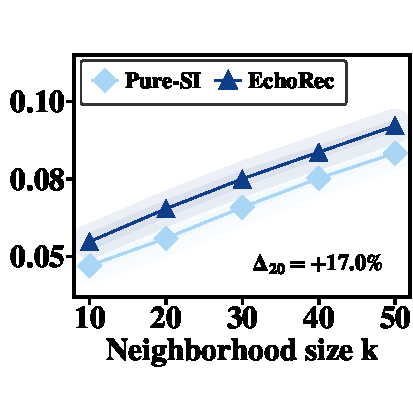
\includegraphics[width=0.468\linewidth]{figure/scientific_sshg_semantic.pdf}\hspace{0.02\linewidth}
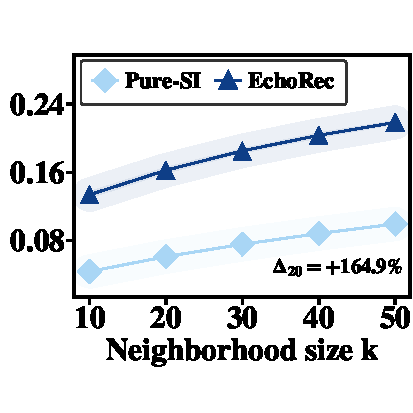
\includegraphics[width=0.468\linewidth]{figure/scientific_sshg_transfer.pdf}}
{\fbox{\rule{0pt}{1.5in}\rule{0.43\linewidth}{0pt}}\hspace{0.02\linewidth}\fbox{\rule{0pt}{1.5in}\rule{0.43\linewidth}{0pt}}}
\caption{Scientific。}
\end{subfigure}
\caption{CDs 与 Scientific 上的受控 SSHG 诊断。上排对应 CDs，下排对应 Scientific；在每一排中，左图跟踪注入前语义对齐，右图跟踪注入后结构迁移。EchoRec 在不同邻域尺度上均稳定优于 Pure-SI。}
\label{fig:cds_scientific_sshg_curves}
\end{figure}

图~\ref{fig:cds_scientific_sshg_curves} 在两个代表性数据集上直观展示了多尺度诊断结果。在 CDs 与 Scientific 上，EchoRec 都同时提升了注入前语义对齐与注入后结构迁移保真度，这与 SSHG 机制所预测的模式一致。以 $k=20$ 为例，在 CDs 上，EchoRec 将语义对齐从 0.033 提升到 0.053，将结构迁移 Jaccard 从 0.115 提升到 0.193；Scientific 上也呈现出相同方向、且幅度更大的改进。附录表~\ref{tab:multidataset_sshg_delta} 进一步将这一受控诊断扩展到四个数据集：所有数据集的 $\Delta$PreAlign@20、$\Delta$Jaccard@20、$\Delta$RBO@20 与 $\Delta$NDCG@10 均为正值。这说明 SACP 稳定地降低了注入前错配，而 SI 则稳定地帮助 LLM 在注入后保留更多局部序列结构。这些基于 overlap 与 order 的指标只是经验代理，而不是附录~\ref{app:theory} 中连续序列保持误差的直接观测，但它们一致地反映了同一个“局部结构保持”机制。

\subsection{RQ4：序列扰动稳定性}
\label{subsec:seq-perturb}

我们进一步测试当输入序列在推理时受到扰动时，EchoRec 是否仍能保持稳定。图~\ref{fig:seq_perturb_panel} 给出了 CDs 与 Scientific 两个数据集上四种设置的结果：原始历史、shuffle、reverse 与 drop-recent。可以看到，在两个数据集上，EchoRec 不仅保持了更强的干净输入性能，而且在 shuffle 与 drop-recent 这类中等强度扰动下通常表现出更小的退化幅度；而两种方法在完全 reverse 情形下都会显著下降。这一现象说明，教师侧预处理提升的是序列利用的稳定性，而不仅仅是放大了脆弱的 prompt 级顺序敏感性。

\begin{figure}[t]
\centering
\IfFileExists{figure/sequence_perturb_panel.pdf}
{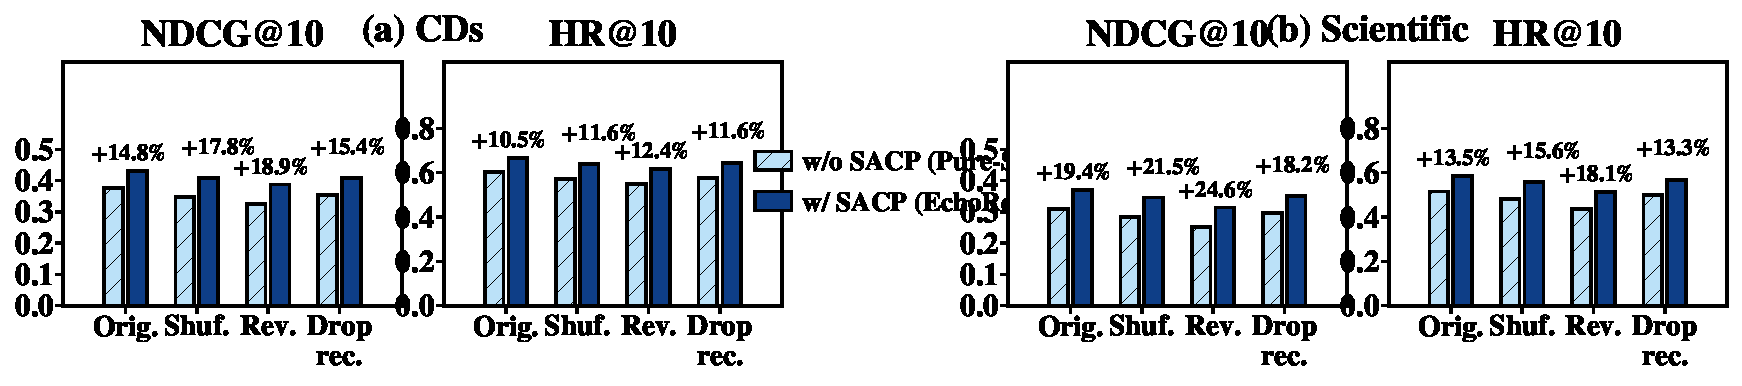
\includegraphics[width=\textwidth]{figure/sequence_perturb_panel.pdf}}
{\fbox{\rule{0pt}{2.2in}\rule{0.98\textwidth}{0pt}}}
\caption{CDs 与 Scientific 上的序列扰动实验结果。}
\label{fig:seq_perturb_panel}
\end{figure}

\section{相关工作}
\label{sec:related}

\subsection{序列推荐}

序列推荐主要关注如何从协同过滤信号中识别相似物品或用户，并建模用户偏好随交互历史的演化。早期方法将矩阵分解与马尔可夫转移结合，以捕捉时间动态，例如 FPMC~\cite{rendle2010fpmc}。随后神经模型推动了这一方向的发展：GRU4Rec~\cite{hidasi2016gru4rec} 使用循环结构建模序列，NextItNet~\cite{yuan2019nextitnet} 引入卷积式序列建模，而后续的 SASRec~\cite{kang2018sasrec} 与 BERT4Rec~\cite{sun2019bert4rec} 则进一步通过注意力架构提升了序列表征能力。近年来，CMCLRec~\cite{xu2024cmclrec}、CLLMRec~\cite{lu2025cllmrec}、HPSERec~\cite{xu2025hpserec} 与 FMLP-Rec~\cite{zhou2022fmlprec} 等工作，又分别从多模态增强、基于 LLM 的视图增强、长尾建模与轻量编码器等方面进一步强化序列学习。尽管如此，序列推荐空间仍主要由 ID 共现与曝光统计塑形，因此在迁移到以 LLM 为中心的语义宿主空间时，往往缺乏足够平滑且兼容的语义结构。

\subsection{基于 LLM 的推荐}

随着大语言模型兴起，推荐研究开始探索如何将 LLM 与序列信号更紧密地耦合~\cite{lin2025survey,zhao2024era}。早期工作主要通过 prompting 或轻量调优来适配 LLM：TALLRec~\cite{bao2023tallrec} 使用 PEFT 连接语言建模与推荐任务，而 ThinkRec~\cite{yu2026thinkrec} 则进一步引入了显式推理。随着纯文本适配的局限逐渐显现，后续研究重新把协同知识引入 LLM 流程。LLaRA~\cite{liao2024llara} 将 CF-SRec 物品嵌入与文本 prompt 结合，CoLLM~\cite{zhang2025collm} 直接把协同嵌入注入在线 LLM 上下文，而 A-LLMRec~\cite{kim2024allmrec} 则通过表示对齐进一步增强协同知识吸收。更近一步，Kim 等人~\cite{kim2025lost} 指出已有 LLM4Rec 模型仍难以真正捕捉交互序列中的动态偏好，并提出 LLM-SRec 进行序列感知蒸馏。另一条路线则使用 LLM 去增强小型推荐器，包括 RLMRec~\cite{ren2024rlmrec}、LRD~\cite{yang2024lrd}、LLM-ESR~\cite{liu2024llmesr}、SRA-CL~\cite{cui2025sracl} 与 LLMEmb~\cite{liu2025llmemb}，而 TCA4Rec~\cite{lin2026tca4rec} 进一步探索了生成空间中更显式的协同对齐。受近期大-小模型协同研究启发~\cite{zhang2026crossscale,lv2025lsc4rec}，我们认为这两条路线不应被割裂地看待。然而，现有方法主要聚焦于注入时的对齐或蒸馏，对注入前教师空间与 LLM 语义宿主之间的结构错配关注不足。

\section{结论}
\label{sec:conclusion}

本文分析了 LLM 增强序列推荐中的\emph{语义-序列异构鸿沟}（SSHG），并提出了 EchoRec，一个围绕“先重塑序列推荐空间，再注入结构感知信号”组织的分阶段协同框架。我们将 SSHG 具体化为局部语义度量错配与语义邻域拓扑碎片化，并设计 SACP 通过 item-level 语义一致性与 user-level 语义平滑在 SI 之前先对教师空间进行净化。在当前实验设置下，EchoRec 相比强基线取得了一致的性能提升；受控诊断进一步表明，EchoRec 能够改善序列推荐空间与语义空间的对齐程度，并在注入 LLM 后更忠实地保留局部序列结构，这些变化也伴随着更好的下游排序结果。总体而言，这些结果支持了一个与理论上“教师空间预对齐 + 注入时漂移控制”共同降低序列保持误差上界相一致的机制解释。

\section{未来工作}
\label{sec:future_work}

一个重要的下一步是将这一分阶段协同框架扩展到更广泛的训练与部署设定。具体而言，值得进一步研究更高效的语义资产构造方式、参数高效的适配策略，以及更广泛的多模态与跨域场景，从而使大-小模型协同在真实推荐流程中同时具备有效性与实用性。

\begin{thebibliography}{99}

\bibitem{xu2025c2lrec}
Xiaolong Xu, Hongsheng Dong, Haolong Xiang, Xiyuan Hu, Xiaoyong Li, Xiaoyu Xia, Xuyun Zhang, Lianyong Qi, and Wanchun Dou. 2025.
C2lRec: Causal Contrastive Learning for User Cold-start Recommendation with Social Variables.
\textit{ACM Transactions on Information Systems} 43, 6 (2025), 143:1--143:28.

\bibitem{xu2024cmclrec}
Xiaolong Xu, Hongsheng Dong, Lianyong Qi, Xuyun Zhang, Haolong Xiang, Xiaoyu Xia, Yanwei Xu, and Wanchun Dou. 2024.
CMCLRec: Cross-modal Contrastive Learning for User Cold-start Sequential Recommendation.
In \textit{Proceedings of the 47th International ACM SIGIR Conference on Research and Development in Information Retrieval (SIGIR '24)}. ACM, 1589--1598.

\bibitem{xu2025hpserec}
Xiaolong Xu, Xudong Zhao, Haolong Xiang, Xuyun Zhang, Wei Shen, Hongsheng Hu, and Lianyong Qi. 2025.
HPSERec: A Hierarchical Partitioning and Stepwise Enhancement Framework for Long-tailed Sequential Recommendation.
In \textit{Advances in Neural Information Processing Systems 39 (NeurIPS '25)}.

\bibitem{lu2025cllmrec}
Fan Lu, Xiaolong Xu, Haolong Xiang, Lianyong Qi, Xiaokang Zhou, Fei Dai, and Wanchun Dou. 2025.
CLLMRec: Contrastive Learning with LLMs-based View Augmentation for Sequential Recommendation.
In \textit{Proceedings of the Thirty-Fourth International Joint Conference on Artificial Intelligence (IJCAI '25)}, 3153--3161.

\bibitem{lin2026tca4rec}
Zhuowei Lin, Huan Yao, Xingchen Ma, Ruiran Yan, Yuxiang Ren, Xian Wu, Zhixiang Zhang, and Yong Li. 2026.
Token-level collaborative alignment for LLM-based generative recommendation.
In \textit{Proceedings of the ACM Web Conference 2026 (WWW '26)}. ACM.

\bibitem{wang2026contextbias}
Yue Wang, Guibiao Wang, Mingde Yao, Jiawei Chen, Xin Xin, and Fuli Feng. 2026.
Does LLM focus on the right words? Mitigating context bias in LLM-based recommenders.
In \textit{Proceedings of the ACM Web Conference 2026 (WWW '26)}. ACM.

\bibitem{yu2026thinkrec}
Qihang Yu, Kairui Fu, Zheqi Lv, Shengyu Zhang, Xinhui Wu, Chen Lin, Feng Wei, Bo Zheng, and Wenwu Ou. 2026.
ThinkRec: Thinking-based recommendation via LLM.
In \textit{Proceedings of the ACM Web Conference 2026 (WWW '26)}. ACM.

\bibitem{zhang2026crossscale}
Yipeng Zhang, Xin Wang, Hong Chen, Junwei Pan, Qian Li, Jun Zhang, Jie Jiang, Hong Mei, and Wenwu Zhu. 2026.
Cross-Scale Collaboration between LLMs and Lightweight Sequential Recommenders with Domain-Specific Latent Reasoning.
In \textit{Proceedings of the AAAI Conference on Artificial Intelligence (AAAI '26)}.

\bibitem{kim2025lost}
Kibum Kim, Hongseok Kang, Sein Kim, Jiwan Kim, Donghyun Kim, Minchul Yang, and Chanyoung Park. 2025.
Lost in sequence: Do large language models understand sequential recommendation?
In \textit{Proceedings of the 31st ACM SIGKDD Conference on Knowledge Discovery and Data Mining (KDD '25)}. ACM.

\bibitem{he2025llm2rec}
Yingzhi He, Xiaohao Liu, An Zhang, Yunshan Ma, and Tat-Seng Chua. 2025.
LLM2Rec: Large language models are powerful embedding models for sequential recommendation.
In \textit{Proceedings of the 31st ACM SIGKDD Conference on Knowledge Discovery and Data Mining (KDD '25)}. ACM.

\bibitem{hong2025eagerllm}
Minjie Hong, Yan Xia, Zehan Wang, Jieming Zhu, Ye Wang, and Sihang Cai. 2025.
EAGER-LLM: Enhancing large language models as recommenders through exogenous behavior-semantic integration.
In \textit{Proceedings of the ACM Web Conference 2025 (WWW '25)}. ACM.

\bibitem{wang2025pad}
Yuhao Wang, Junwei Pan, Pengyue Jia, Wanyu Wang, Maolin Wang, Zhixiang Feng, Xiaotian Li, Jie Jiang, and Xiangyu Zhao. 2025.
Pre-train, align, and disentangle: Empowering sequential recommendation with large language models.
In \textit{Proceedings of the 48th International ACM SIGIR Conference on Research and Development in Information Retrieval (SIGIR '25)}. ACM.

\bibitem{cui2025sracl}
Ziqiang Cui, Yunpeng Weng, Xing Tang, Xiaokun Zhang, Shiwei Li, Peiyang Liu, Bowei He, Dugang Liu, Weihong Luo, Xiuqiang He, and Chen Ma. 2025.
SRA-CL: Semantic retrieval augmented contrastive learning for sequential recommendation.
In \textit{Advances in Neural Information Processing Systems 39 (NeurIPS '25)}.

\bibitem{lv2025lsc4rec}
Zheqi Lv, Hongyan Zhao, Han Wang, Yang Song, Yongsheng Zhang, Yuxiang Wang, and Dawei Yin. 2025.
Collaboration of large language models and small recommendation models for device-cloud recommendation.
In \textit{Proceedings of the 31st ACM SIGKDD Conference on Knowledge Discovery and Data Mining (KDD '25)}. ACM.

\bibitem{zhang2025collm}
Shuai Zhang, Keqin Bao, Yang Zhang, Yunxin Hu, Fuli Feng, Xiangnan He, and Xiang Wang. 2025.
CoLLM: Integrating collaborative embeddings into large language models for recommendation.
\textit{IEEE Transactions on Knowledge and Data Engineering} 37, 2 (2025), 1037--1051.

\bibitem{lin2025survey}
Jianghao Lin, Xinyi Dai, Yunjia Xi, Weiwen Liu, Bo Chen, Hao Zhang, Yong Liu, Chuhan Wu, Xiangyang Li, Chenxu Zhu, Huifeng Guo, Yong Yu, Ruiming Tang, and Weinan Zhang. 2025.
How can recommender systems benefit from large language models: A survey.
\textit{ACM Transactions on Information Systems} 43, 2 (2025), Article 28.

\bibitem{liu2025llmemb}
Qidong Liu, Xian Wu, Wanyu Wang, Yejing Wang, Yuanshao Zhu, Xiangyu Zhao, Feng Tian, and Yefeng Zheng. 2025.
LLMEmb: Large language model can be a good embedding generator for sequential recommendation.
In \textit{Proceedings of the AAAI Conference on Artificial Intelligence (AAAI '25)}.

\bibitem{wang2025piccdr}
Ke Wang, Ji Zhang, and Kuan Liu. 2025.
Enhancing cross-domain recommendation with plug-in contrastive representations from large language models.
In \textit{Proceedings of the 48th International ACM SIGIR Conference on Research and Development in Information Retrieval (SIGIR '25)}. ACM.

\bibitem{liao2024llara}
Zhiyu Liao, Xujiang Zhao, Le Wu, Jingjing Li, Xing Xie, and Peng Cui. 2024.
LLaRA: Large language-recommendation assistant.
In \textit{Proceedings of the 47th International ACM SIGIR Conference on Research and Development in Information Retrieval (SIGIR '24)}. ACM.

\bibitem{kim2024allmrec}
Sein Kim, Hongseok Kang, Seungyoon Choi, Donghyun Kim, Minchul Yang, and Chanyoung Park. 2024.
Large language models meet collaborative filtering: An efficient all-round LLM-based recommender system.
In \textit{Proceedings of the 30th ACM SIGKDD Conference on Knowledge Discovery and Data Mining (KDD '24)}. ACM.

\bibitem{ren2024rlmrec}
Xubin Ren, Wei Wei, Lianghao Xia, Lixin Su, Suqi Cheng, Junfeng Wang, Dawei Yin, and Chao Huang. 2024.
Representation learning with large language models for recommendation.
In \textit{Proceedings of the ACM Web Conference 2024 (WWW '24)}. ACM, 3461--3472.

\bibitem{liu2024llmesr}
Qidong Liu, Xian Wu, Yejing Wang, Zijian Zhang, Feng Tian, Yefeng Zheng, and Xiangyu Zhao. 2024.
LLM-ESR: Large language models enhancement for long-tailed sequential recommendation.
In \textit{Advances in Neural Information Processing Systems 38 (NeurIPS '24)}.

\bibitem{yang2024lrd}
Shenghao Yang, Weizhi Ma, Peijie Sun, Qingyao Ai, Yiqun Liu, Mingchen Cai, and Min Zhang. 2024.
Sequential recommendation with latent relations based on large language model.
In \textit{Proceedings of the 47th International ACM SIGIR Conference on Research and Development in Information Retrieval (SIGIR '24)}. ACM.

\bibitem{zheng2024lcrec}
Bowen Zheng, Yupeng Hou, Hongyu Lu, Yu Chen, Wayne Xin Zhao, Ming Chen, and Ji-Rong Wen. 2024.
Adapting large language models by integrating collaborative semantics for recommendation.
In \textit{Proceedings of the 40th IEEE International Conference on Data Engineering (ICDE '24)}. IEEE, 1435--1448.

\bibitem{zheng2024trsr}
Zhi Zheng, Wenshuo Chao, Zhaopeng Qiu, Hengshu Zhu, and Hui Xiong. 2024.
Harnessing large language models for text-rich sequential recommendation.
In \textit{Proceedings of the ACM Web Conference 2024 (WWW '24)}. ACM, 3207--3216.

\bibitem{wu2024coral}
Junda Wu, Cheng-Chun Chang, Tong Yu, Zhankui He, Jianing Wang, Yupeng Hou, and Julian McAuley. 2024.
Coral: Collaborative retrieval-augmented large language models improve long-tail recommendation.
In \textit{Proceedings of the 30th ACM SIGKDD Conference on Knowledge Discovery and Data Mining (KDD '24)}. ACM, 3391--3401.

\bibitem{zhao2024era}
Zhe Zhao, Wei Fan, Junhao Li, Yuyang Liu, Xing Mei, Yongfeng Wang, Zhiqi Wen, Feng Wang, Xiangyu Zhao, and Ji-Rong Wen et al. 2024.
Recommender systems in the era of large language models (LLMs).
\textit{IEEE Transactions on Knowledge and Data Engineering} (2024).

\bibitem{sun2019bert4rec}
Fei Sun, Jun Liu, Jian Wu, Changhua Pei, Xiao Lin, Wenwu Ou, and Peng Jiang. 2019.
BERT4Rec: Sequential recommendation with bidirectional encoder representations from transformer.
In \textit{Proceedings of the 28th ACM International Conference on Information and Knowledge Management (CIKM '19)}. ACM.

\bibitem{kang2018sasrec}
Wang-Cheng Kang and Julian McAuley. 2018.
Self-attentive sequential recommendation.
In \textit{Proceedings of the 18th IEEE International Conference on Data Mining (ICDM '18)}. IEEE.

\bibitem{hidasi2016gru4rec}
Bal\'azs Hidasi, Alexandros Karatzoglou, Linas Baltrunas, and Domonkos Tikk. 2016.
Session-based recommendations with recurrent neural networks.
In \textit{Proceedings of the 4th International Conference on Learning Representations (ICLR '16)}.

\bibitem{yuan2019nextitnet}
Fajie Yuan, Xiangnan He, Alexandros Karatzoglou, and Lizi Zhang. 2019.
A simple convolutional generative network for next item recommendation.
In \textit{Proceedings of the Twelfth ACM International Conference on Web Search and Data Mining (WSDM '19)}. ACM.

\bibitem{rendle2010fpmc}
Steffen Rendle, Christoph Freudenthaler, and Lars Schmidt-Thieme. 2010.
Factorizing personalized Markov chains for next-basket recommendation.
In \textit{Proceedings of the 19th International Conference on World Wide Web (WWW '10)}. ACM, 811--820.

\bibitem{chen2022iclrec}
Yongjun Chen, Zhiwei Liu, Jia Li, Julian McAuley, and Caiming Xiong. 2022.
Intent contrastive learning for sequential recommendation.
In \textit{Proceedings of the ACM Web Conference 2022 (WWW '22)}. ACM, 2172--2182.

\bibitem{zhou2022fmlprec}
Kun Zhou, Hui Wang, Wayne Xin Zhao, and Ji-Rong Wen. 2022.
Filter-enhanced MLP is all you need for sequential recommendation.
In \textit{Proceedings of the ACM Web Conference 2022 (WWW '22)}. ACM, 2388--2399.

\bibitem{bao2023tallrec}
Keqin Bao, Jizhi Zhang, Yang Zhang, Wenjie Wang, Fuli Feng, and Xiangnan He. 2023.
TALLRec: An effective and efficient tuning framework to align large language model with recommendation.
In \textit{Proceedings of the 17th ACM Conference on Recommender Systems (RecSys '23)}. ACM.

\end{thebibliography}

\input{checklist}

\appendix

\section{理论分析：为什么降低 SSHG 能提升序列保持}
\label{app:theory}

为了形式化 EchoRec 所期望实现的机制，我们从局部邻域分布的角度分析跨空间迁移。我们的目的不是为任意迁移系统声称一个普适定律，而是在显式的语义宿主兼容性假设下，给出一个\emph{条件机制定理}。

\subsection{分布设定}
\label{app:theory_setup}

对于每个用户 $u$，记 $\mathcal{N}_u^K$ 为大小为 $K$ 的\emph{共享候选池}。需要强调的是，$\mathcal{N}_u^K$ 并不是在不同空间中分别构造出的硬 Top-$K$ 集合，而是一个预先固定的共享候选池，所有邻域分布都定义在这一共同支持集上。

对于每个空间 $a \in \{\mathrm{sem}, \mathrm{seq}, \mathrm{llm}\}$，记 $s_u^a(v)$ 为该空间对候选 $v \in \mathcal{N}_u^K$ 分配的邻域分数。相应的 soft 邻域分布定义为
\begin{equation}
p_u^a(v)
=
\frac{\exp(s_u^a(v)/\tau)}
{\sum_{v' \in \mathcal{N}_u^K}\exp(s_u^a(v')/\tau)},
\qquad
a \in \{\mathrm{sem}, \mathrm{seq}, \mathrm{llm}\},
\label{eq:soft_dist}
\end{equation}
其中，$p_u^a(v)$ 表示空间 $a$ 中用户 $u$ 对候选 $v$ 分配的概率，$s_u^a(v)$ 为对应的邻域分数，$\tau>0$ 为 softmax 温度。因此，$p_u^{sem}$、$p_u^{seq}$ 与 $p_u^{llm}$ 都是在同一支持集 $\mathcal{N}_u^K$ 上的严格正分布。对于 LLM 侧，$s_u^{llm}(j)$ 由阶段二的检索分数 Eq.~\eqref{eq:stage2_score} 实例化；对于教师侧，$s_u^{seq}(v)$ 则表示增强教师在同一候选池上的打分。

我们将总变差距离定义为
\begin{equation}
TV(p,q):=\frac{1}{2}\|p-q\|_1.
\label{eq:tv_def}
\end{equation}
其中，$p$ 与 $q$ 是定义在同一支持集上的分布。
我们关心的核心量是\emph{序列保持误差}
\begin{equation}
\mathcal{E}_{ret}(u):=TV(p_u^{seq},p_u^{llm}),
\label{eq:ret_error}
\end{equation}
它衡量的是教师侧局部序列结构在注入 LLM 空间后丢失了多少。

对于对齐项，我们定义一阶对齐强度
\begin{equation}
E_{align}:=\frac{1}{|\mathcal U|}\sum_{u\in\mathcal U}\|\overline{\mathbf{u}}_u-\overline{\mathbf{t}}_u\|_2,
\label{eq:e_align}
\end{equation}
其中，$\overline{\mathbf{u}}_u$ 与 $\overline{\mathbf{t}}_u$ 分别表示 Eq.~\eqref{eq:stage2_score} 与 Eq.~\eqref{eq:stage2_match} 所使用共享检索子空间中的归一化 LLM 用户表示与归一化教师用户表示。实际优化目标中使用的是平方距离形式
\begin{equation}
L_{align}:=\frac{1}{|\mathcal U|}\sum_{u\in\mathcal U}\|\overline{\mathbf{u}}_u-\overline{\mathbf{t}}_u\|_2^2.
\label{eq:l_align}
\end{equation}
由 Jensen 不等式，或等价地由 Cauchy--Schwarz 不等式，有
\begin{equation}
E_{align}\le \sqrt{L_{align}}.
\label{eq:e_vs_l_align}
\end{equation}
因此，在实际目标中压低平方距离项，也会同步压低下文定理中的对齐项。

\subsection{结构性假设}
\label{app:theory_assumptions}

下面给出形式化 EchoRec 机制所需的结构性假设。

\paragraph{假设 A.1（教师侧与 LLM 侧的局部决策规则）。}
对于每个用户 $u$，存在两个局部分布映射
\begin{equation}
\Phi_u^{seq}:\mathbb{R}^d\to\Delta^K,
\qquad
\Phi_u^{llm}:\mathbb{R}^d\to\Delta^K,
\label{eq:two_maps}
\end{equation}
其中，$\Delta^K$ 表示定义在共享候选池上的 $K$ 维概率单纯形，$d$ 为共享检索子空间的维度，并满足
\begin{equation}
p_u^{seq}=\Phi_u^{seq}(\overline{\mathbf{t}}_u),
\qquad
p_u^{llm}=\Phi_u^{llm}(\overline{\mathbf{u}}_u).
\label{eq:map_outputs}
\end{equation}
其中，$\Phi_u^{seq}$ 描述教师侧的局部决策规则，而 $\Phi_u^{llm}$ 描述注入后 LLM 侧的局部决策规则。

\paragraph{假设 A.2（语义宿主兼容性的建模假设）。}
我们假设，对于固定的教师表示 $\overline{\mathbf{t}}_u$，教师侧与 LLM 侧邻域规则之间的差异，可以由重塑后教师结构与冻结语义参考之间的残余错配上界：
\begin{equation}
\|\Phi_u^{seq}(\overline{\mathbf{t}}_u)-\Phi_u^{llm}(\overline{\mathbf{t}}_u)\|_1
\le
C_{m,u}\,TV(p_u^{seq},p_u^{sem}).
\label{eq:compat_user}
\end{equation}
其中，$C_{m,u}>0$ 衡量用户级语义宿主兼容性对残余语义-序列错配的敏感程度。
为简化表述，我们定义统一常数
\begin{equation}
C_m:=\sup_{u\in\mathcal U} C_{m,u},
\label{eq:compat_uniform_const}
\end{equation}
从而有
\begin{equation}
\|\Phi_u^{seq}(\overline{\mathbf{t}}_u)-\Phi_u^{llm}(\overline{\mathbf{t}}_u)\|_1
\le
C_m\,TV(p_u^{seq},p_u^{sem}).
\label{eq:compat_uniform}
\end{equation}
这是一项\emph{结构性建模假设}，而不是由具体架构直接推出的性质。它刻画的是 SSHG 在语义宿主兼容性情形下的作用：如果重塑后的教师仍然与冻结语义参考相距较远，那么即使输入的是相同的教师表示，LLM 侧局部决策规则也无法忠实复现教师侧邻域结构。因此，这一假设应被理解为一种用于编码宿主兼容机制的抽象建模，而非架构或训练目标的直接推论。

\paragraph{假设 A.3（注入时的 Lipschitz 稳定性）。}
LLM 侧局部决策映射关于用户表示是 $C_\Phi$-Lipschitz 的，即
\begin{equation}
\|\Phi_u^{llm}(\mathbf{h})-\Phi_u^{llm}(\mathbf{h}')\|_1
\le
C_\Phi\|\mathbf{h}-\mathbf{h}'\|_2,
\qquad
\forall \mathbf{h},\mathbf{h}'\in\mathbb R^d.
\label{eq:lipschitz_llm}
\end{equation}
其中，$C_\Phi>0$ 为 LLM 侧局部决策映射的 Lipschitz 常数。该假设表示：如果阶段二能够让注入后的 LLM 表示保持接近教师表示，那么由此诱导的 LLM 邻域分布也不会发生过度漂移。

\subsection{主定理：序列保持误差上界}
\label{app:main_theorem}

\begin{theorem}[序列保持误差上界]
\label{thm:retention}
在假设 A.1--A.3 下，对于任意用户 $u$，
\begin{equation}
TV(p_u^{seq},p_u^{llm})
\le
\frac{C_m}{2}\,TV(p_u^{seq},p_u^{sem})
+
\frac{C_\Phi}{2}\,\|\overline{\mathbf{t}}_u-\overline{\mathbf{u}}_u\|_2.
\label{eq:user_bound}
\end{equation}
对所有用户取平均可得
\begin{equation}
\frac{1}{|\mathcal U|}\sum_{u\in\mathcal U}TV(p_u^{seq},p_u^{llm})
\le
\frac{C_m}{2}\,\bar m
+
\frac{C_\Phi}{2}\,E_{align},
\label{eq:avg_bound}
\end{equation}
其中
\begin{equation}
\bar m:=\frac{1}{|\mathcal U|}\sum_{u\in\mathcal U}TV(p_u^{seq},p_u^{sem}).
\label{eq:mbar}
\end{equation}
进一步利用 Eq.~\eqref{eq:e_vs_l_align}，可得
\begin{equation}
\frac{1}{|\mathcal U|}\sum_{u\in\mathcal U}TV(p_u^{seq},p_u^{llm})
\le
\frac{C_m}{2}\,\bar m
+
\frac{C_\Phi}{2}\,\sqrt{L_{align}}.
\label{eq:avg_bound_lalign}
\end{equation}
\end{theorem}

\begin{proof}
由 Eq.~\eqref{eq:map_outputs}，
\begin{equation}
p_u^{seq}=\Phi_u^{seq}(\overline{\mathbf{t}}_u),
\qquad
p_u^{llm}=\Phi_u^{llm}(\overline{\mathbf{u}}_u).
\label{eq:proof_start}
\end{equation}
因此，
\begin{align}
\|p_u^{seq}-p_u^{llm}\|_1
&=
\|\Phi_u^{seq}(\overline{\mathbf{t}}_u)-\Phi_u^{llm}(\overline{\mathbf{u}}_u)\|_1 \notag\\
&\le
\|\Phi_u^{seq}(\overline{\mathbf{t}}_u)-\Phi_u^{llm}(\overline{\mathbf{t}}_u)\|_1
+
\|\Phi_u^{llm}(\overline{\mathbf{t}}_u)-\Phi_u^{llm}(\overline{\mathbf{u}}_u)\|_1,
\label{eq:triangle_maps}
\end{align}
该不等式由三角不等式得到。

第一项由假设 A.2 控制：
\begin{equation}
\|\Phi_u^{seq}(\overline{\mathbf{t}}_u)-\Phi_u^{llm}(\overline{\mathbf{t}}_u)\|_1
\le
C_m\,TV(p_u^{seq},p_u^{sem}).
\label{eq:first_term}
\end{equation}
第二项由假设 A.3 控制：
\begin{equation}
\|\Phi_u^{llm}(\overline{\mathbf{t}}_u)-\Phi_u^{llm}(\overline{\mathbf{u}}_u)\|_1
\le
C_\Phi\|\overline{\mathbf{t}}_u-\overline{\mathbf{u}}_u\|_2.
\label{eq:second_term}
\end{equation}
将 Eq.~\eqref{eq:first_term} 与 Eq.~\eqref{eq:second_term} 代入 Eq.~\eqref{eq:triangle_maps}，可得
\begin{equation}
\|p_u^{seq}-p_u^{llm}\|_1
\le
C_m\,TV(p_u^{seq},p_u^{sem})
+
C_\Phi\|\overline{\mathbf{t}}_u-\overline{\mathbf{u}}_u\|_2.
\label{eq:l1_bound}
\end{equation}
根据 Eq.~\eqref{eq:tv_def} 中总变差距离的定义，
\begin{equation}
TV(p_u^{seq},p_u^{llm})
=
\frac{1}{2}\|p_u^{seq}-p_u^{llm}\|_1
\le
\frac{C_m}{2}\,TV(p_u^{seq},p_u^{sem})
+
\frac{C_\Phi}{2}\,\|\overline{\mathbf{t}}_u-\overline{\mathbf{u}}_u\|_2,
\end{equation}
即得 Eq.~\eqref{eq:user_bound}。

对 Eq.~\eqref{eq:user_bound} 在所有用户上取平均，有
\begin{align}
\frac{1}{|\mathcal U|}\sum_{u\in\mathcal U}TV(p_u^{seq},p_u^{llm})
&\le
\frac{C_m}{2}\cdot
\frac{1}{|\mathcal U|}\sum_{u\in\mathcal U}TV(p_u^{seq},p_u^{sem})
+
\frac{C_\Phi}{2}\cdot
\frac{1}{|\mathcal U|}\sum_{u\in\mathcal U}\|\overline{\mathbf{t}}_u-\overline{\mathbf{u}}_u\|_2 \notag\\
&=
\frac{C_m}{2}\,\bar m+\frac{C_\Phi}{2}\,E_{align},
\end{align}
从而得到 Eq.~\eqref{eq:avg_bound}。最后，再利用 Eq.~\eqref{eq:e_vs_l_align} 即可得到 Eq.~\eqref{eq:avg_bound_lalign}。
\end{proof}

\paragraph{解释。}
定理~\ref{thm:retention} 表明，最终的序列保持误差由两个来源共同决定：一是注入前错配项 $TV(p_u^{seq},p_u^{sem})$，它刻画了阶段一之后重塑教师与冻结语义参考之间还剩下多少差距；二是注入时漂移项 $\|\overline{\mathbf{t}}_u-\overline{\mathbf{u}}_u\|_2$，它刻画了阶段二中注入后的 LLM 表示偏离教师对齐子空间的程度。因此，阶段一通过将教师空间拉向冻结语义参考来降低前者，阶段二则通过显式教师对齐来降低后者。两者共同作用，从而压缩序列保持误差的上界。

\subsection{与主文诊断实验的关系}
\label{app:diagnosis_relation}

上述理论分析是以连续的局部邻域分布与 TV 型保持误差为对象进行的。在实验中，这些量无法从最终排序结果中被直接观测。因此，主文采用了如 Jaccard@k 与 RBO@20 这样的 overlap 与 order 代理指标来诊断同一潜在现象，即\emph{局部结构保持}。也就是说，理论中的保持误差与实验中的结构迁移保真度并不是数值上一一对应的量，但它们描述的是同一个机制在不同抽象层次下的表现。

\subsection{讨论：与扰动稳定性的关系}
\label{app:perturb_cor}

主文显示，EchoRec 在 \emph{shuffle} 与 \emph{drop-recent} 这类中等强度扰动下更稳定。即使在完全 reverse 的情况下，EchoRec 的退化也仍小于 Pure-SI，这与一种“对序列顺序更敏感、但对迁移扭曲不那么脆弱”的模型行为是一致的。

从上文相同的分布视角出发，这一现象是自然的。如果教师侧错配在注入前更小、注入时漂移控制得更好，那么被迁移过去的序列结构在干净输入下就会更连贯，也更不容易在中等强度扰动下发生塌缩。这有助于解释为什么 EchoRec 在 \emph{shuffle} 与 \emph{drop-recent} 下表现出更小的退化。

与此同时，\emph{reverse} 下 EchoRec 依然会发生变化，并不应被看作矛盾。恰恰相反，这说明模型仍然保留了有意义的顺序敏感性，而不是退化成一种伪顺序不变的行为。因此，我们更倾向于将扰动实验视为一种定性的机制证据：更干净的教师空间与更受控的注入过程，会带来更稳定、但仍然保留顺序感知能力的 LLM 表示。

\section{补充实验设置}
\label{app:exp_settings}

\subsection{数据集}
\label{app:datasets}

遵循 Kim 等人~\cite{kim2025lost} 的共享 benchmark，我们使用四个 Amazon five-core 数据集，分别是 Movies、Scientific、Electronics 与 CDs。预处理后，每个数据集均仅保留至少具有 5 次交互的用户与物品。表~\ref{tab:dataset_stats} 总结了本文使用的 benchmark 统计信息。

\begin{table}[H]
\centering
\caption{共享 benchmark 协议下的数据集统计信息。}
\label{tab:dataset_stats}
\small
\setlength{\tabcolsep}{7pt}
\renewcommand{\arraystretch}{1.1}
\begin{tabular}{lrrrr}
\toprule
Dataset & \#Users & \#Items & \#Interactions & Sparsity \\
\midrule
Movies & 11,947 & 17,490 & 144,071 & 99.93\% \\
Scientific & 23,627 & 25,764 & 266,164 & 99.96\% \\
Electronics & 27,601 & 31,533 & 292,308 & 99.97\% \\
CDs & 18,481 & 30,951 & 284,695 & 99.95\% \\
\bottomrule
\end{tabular}
\end{table}

\subsection{对比方法}
\label{app:baselines}

\noindent 在共享 retrieval-style 协议下，我们选取 9 个可直接比较的方法作为基线。
\begin{itemize}[leftmargin=1.5em]
\item \textbf{GRU4Rec} 通过循环神经网络建模交互序列中的短程转移动态~\cite{hidasi2016gru4rec}。
\item \textbf{BERT4Rec} 采用双向 Transformer 与 masked-item prediction 学习上下文感知的序列表征~\cite{sun2019bert4rec}。
\item \textbf{NextItNet} 是一个基于空洞残差卷积块的自回归序列推荐器，用于下一物品预测~\cite{yuan2019nextitnet}。
\item \textbf{SASRec} 利用 self-attention 捕捉用户行为序列中最相关的依赖关系，并作为本文中的 vanilla 基线~\cite{kang2018sasrec}。
\item \textbf{TALLRec} 主要通过轻量调优和文本 prompt 使 LLM 适配推荐任务~\cite{bao2023tallrec}。
\item \textbf{LLaRA} 通过 assistant-style 流程将推荐信号组织为指令式交互，使 LLM 保持在推荐回路中~\cite{liao2024llara}。
\item \textbf{A-LLMRec} 通过推荐器与语言模型之间的高效表示对齐，将协同过滤信号迁移到 LLM~\cite{kim2024allmrec}。
\item \textbf{CoLLM} 将协同物品嵌入直接注入 LLM，使推荐推理同时利用语义上下文与协同线索~\cite{zhang2025collm}。
\item \textbf{LLM-SRec} 将序列感知嵌入注入与教师引导表示匹配结合起来，使在线 LLM 更忠实地吸收来自预训练序列推荐器的序列信号~\cite{kim2025lost}。
\end{itemize}
这些方法共同覆盖了传统序列建模、prompt tuning、协同对齐、特征注入与序列蒸馏等代表性方向，因此构成了与 EchoRec 最相关的比较对象。

\subsection{实现细节}
\label{app:implementation}

本文所有实验均在配备两张 NVIDIA GeForce RTX 5090 GPU 的工作站上完成。这里进一步说明：表~\ref{tab:main_overall} 中的 \texttt{SASRec} 列始终表示 vanilla \texttt{SASRec} 基线；而 EchoRec 在两阶段训练中使用的是语义对齐 Transformer（\texttt{SA-Transformer}）。这种区分与本文中的角色分工一致：前者用于保持与既有方法的可比性，后者用于承载教师空间重塑。阶段一通过 SACP 重塑教师空间，阶段二固定 LLM，仅优化轻量投影器、对齐映射器与检索头。实际训练中，教师预训练与 SI 训练均在同一双 5090 平台上运行；单卡任务使用一张卡，多卡任务使用两张卡。SI 设 $\lambda_m=1.0$，代码中由 \texttt{--match\_weight} 控制。其余超参数遵循主文与公开训练脚本中的 benchmark 设置。

\paragraph{Prompt 模板。}
为了兼顾复现性与版面整洁，我们保留 prompt 模板，但改成更紧凑的呈现方式，并将语义资产构造与序列注入两类 prompt 分开给出。

\begin{table}[t]
\centering
\caption{阶段一语义资产构造所使用的紧凑版 prompt 模板。这些 prompt 仅用于构建离线语义资产与语义邻域图。}
\label{tab:semantic_asset_prompt_template}
\small
\setlength{\tabcolsep}{6pt}
\renewcommand{\arraystretch}{1.16}
\begin{tabularx}{\textwidth}{>{\bfseries\raggedright\arraybackslash}p{1.15cm} >{\ttfamily\footnotesize\raggedright\arraybackslash}X}
\toprule
Side & Prompt template \\
\midrule
User &
User <user\_id> recently interacted with: <title\_1>, <title\_2>, \ldots, <title\_m>. \\
Item &
Item <item\_id>: <title>. Description: <description>. \\
\bottomrule
\end{tabularx}
\end{table}

\begin{table}[t]
\centering
\caption{阶段二序列注入所使用的紧凑版 prompt 模板。投影后的协同嵌入被插入 \texttt{[HistoryEmb]}，最终表示从 \texttt{[UserOut]} 与 \texttt{[ItemOut]} 读取。}
\label{tab:si_prompt_template}
\small
\setlength{\tabcolsep}{6pt}
\renewcommand{\arraystretch}{1.16}
\begin{tabularx}{\textwidth}{>{\bfseries\raggedright\arraybackslash}p{1.15cm} >{\ttfamily\footnotesize\raggedright\arraybackslash}X}
\toprule
Side & Prompt template \\
\midrule
User &
This user has made a series of purchases in the following order: Item No.1, Time: <t\_1>, "<title\_1>"[HistoryEmb], Item No.2, Time: <t\_2>, "<title\_2>"[HistoryEmb], \ldots, Item No.T, Time: <t\_T>, "<title\_T>"[HistoryEmb]. Based on this sequence of purchases, generate user representation token:[UserOut] \\
Item &
The item title and item embedding are as follows: "<title\_j>"[HistoryEmb], then generate item representation token:[ItemOut] \\
\bottomrule
\end{tabularx}
\end{table}

\section{补充实验结果}
\label{app:extra_results}

\subsection{受控 SSHG 诊断}
\label{app:prelim_extra}

我们在附录中只保留跨数据集汇总，以便附录结构与主文中的机制主线保持一致。具体而言，这里保留最直接支撑 SSHG 机制链条的四个量：注入前语义对齐、注入后结构迁移的 Jaccard@20 与 RBO@20，以及下游 \texttt{NDCG@10} 提升。为了在保持直接可比性的同时进一步提高信息密度，我们将汇总表转为横向布局，并并排报告每个数据集上的 Pure-SI、EchoRec 与相对提升。

\begin{table}[H]
\centering
\caption{跨数据集的受控 SSHG 诊断。对每个指标与数据集，同时报告 Pure-SI、EchoRec 以及 EchoRec 相对 Pure-SI 的相对提升。}
\label{tab:multidataset_sshg_delta}
\small
\setlength{\tabcolsep}{3.6pt}
\renewcommand{\arraystretch}{1.26}
\begingroup
\setlength{\aboverulesep}{0pt}
\setlength{\belowrulesep}{0pt}
\resizebox{\textwidth}{!}{%
\begin{tabular}{
>{\centering\arraybackslash}m{1.90cm}|
ccc||ccc||ccc||ccc}
\toprule
\multirow{2}{*}[-0.35ex]{\shortstack[c]{\textbf{Metric}}}
& \multicolumn{3}{c||}{\textbf{Movies}}
& \multicolumn{3}{c||}{\textbf{Scientific}}
& \multicolumn{3}{c||}{\textbf{Electronics}}
& \multicolumn{3}{c}{\textbf{CDs}} \\
\cmidrule(lr){2-4}\cmidrule(lr){5-7}\cmidrule(lr){8-10}\cmidrule(lr){11-13}
& \textbf{Pure-SI} & \textbf{EchoRec} & \impcell{\textbf{Improv.}}
& \textbf{Pure-SI} & \textbf{EchoRec} & \impcell{\textbf{Improv.}}
& \textbf{Pure-SI} & \textbf{EchoRec} & \impcell{\textbf{Improv.}}
& \textbf{Pure-SI} & \textbf{EchoRec} & \impcell{\textbf{Improv.}} \\
\specialrule{0.42pt}{0pt}{0pt}
PreAlign@20
& 0.0245 & 0.0471 & \impcell{\textbf{+92.4\%}}
& 0.0276 & 0.0654 & \impcell{\textbf{+136.7\%}}
& 0.0166 & 0.0500 & \impcell{\textbf{+200.4\%}}
& 0.0331 & 0.0535 & \impcell{\textbf{+61.6\%}} \\
Jaccard@20
& 0.0529 & 0.1053 & \impcell{\textbf{+99.0\%}}
& 0.0790 & 0.1625 & \impcell{\textbf{+105.6\%}}
& 0.0415 & 0.0850 & \impcell{\textbf{+104.8\%}}
& 0.1155 & 0.1934 & \impcell{\textbf{+67.5\%}} \\
RBO@20
& 0.0544 & 0.1234 & \impcell{\textbf{+126.9\%}}
& 0.0995 & 0.1885 & \impcell{\textbf{+89.4\%}}
& 0.0541 & 0.1036 & \impcell{\textbf{+91.3\%}}
& 0.1297 & 0.2283 & \impcell{\textbf{+75.9\%}} \\
NDCG@10
& 0.3657 & 0.4088 & \impcell{\textbf{+11.8\%}}
& 0.3137 & 0.3797 & \impcell{\textbf{+21.0\%}}
& 0.2736 & 0.3313 & \impcell{\textbf{+21.1\%}}
& 0.3718 & 0.4275 & \impcell{\textbf{+15.0\%}} \\
\bottomrule
\end{tabular}}
\endgroup
\end{table}

表~\ref{tab:multidataset_sshg_delta} 表明，这一机制趋势在四个数据集上都成立。PreAlign@20、Jaccard@20、RBO@20 与 NDCG@10 在所有数据集上的相对提升均为正值，说明 SACP 稳定地降低了注入前语义-序列错配，而 SI 在注入后更忠实地保留了教师侧局部结构。把基线值与相对提升同时写出来后，也更容易看出这种机制收益并不依赖某一个“容易”的数据集：无论是 overlap/order 诊断还是最终排序表现，都呈现出一致的跨数据集改善。

\section{局限性}
\label{app:limitations}

相比单阶段的直接注入流程，EchoRec 带来了更高的训练开销，因为它需要离线语义资产构建、教师侧重塑以及第二阶段 SI 训练。此外，当前评测主要基于共享 retrieval-style benchmark；同样的分阶段设计在更宽松的训练预算、不同的服务约束以及更丰富的多模态场景下会呈现怎样的行为，仍有待后续研究。

\ifPDFTeX
\end{CJK*}
\fi
\end{document}
